\documentclass{article}
\usepackage{epsfig}
\usepackage{graphicx}
\usepackage[top=0.50in, bottom=0.50in, left=0.65in, right=0.75in]{geometry}
%\usepackage[a4paper, total={6in, 10in}]{geometry}
\usepackage[table]{xcolor}
\usepackage{tikz}
\usepackage{algorithm}
\usepackage{mathtools}
\usepackage{amsmath,amssymb}
\usepackage[]{algpseudocode}
\usepackage{enumitem}
\title{CS345 Theoretical Assignment 4 \\ }
\author{\vspace{2mm} \large Ayush Agarwal, 13180 \\ M.Arunothia, 13378}
\date{}
\begin{document}
\maketitle
\tableofcontents
\newpage
\section{Any Guarantee of our First-Attempt Algorithm}
\subsection{Counter Example}
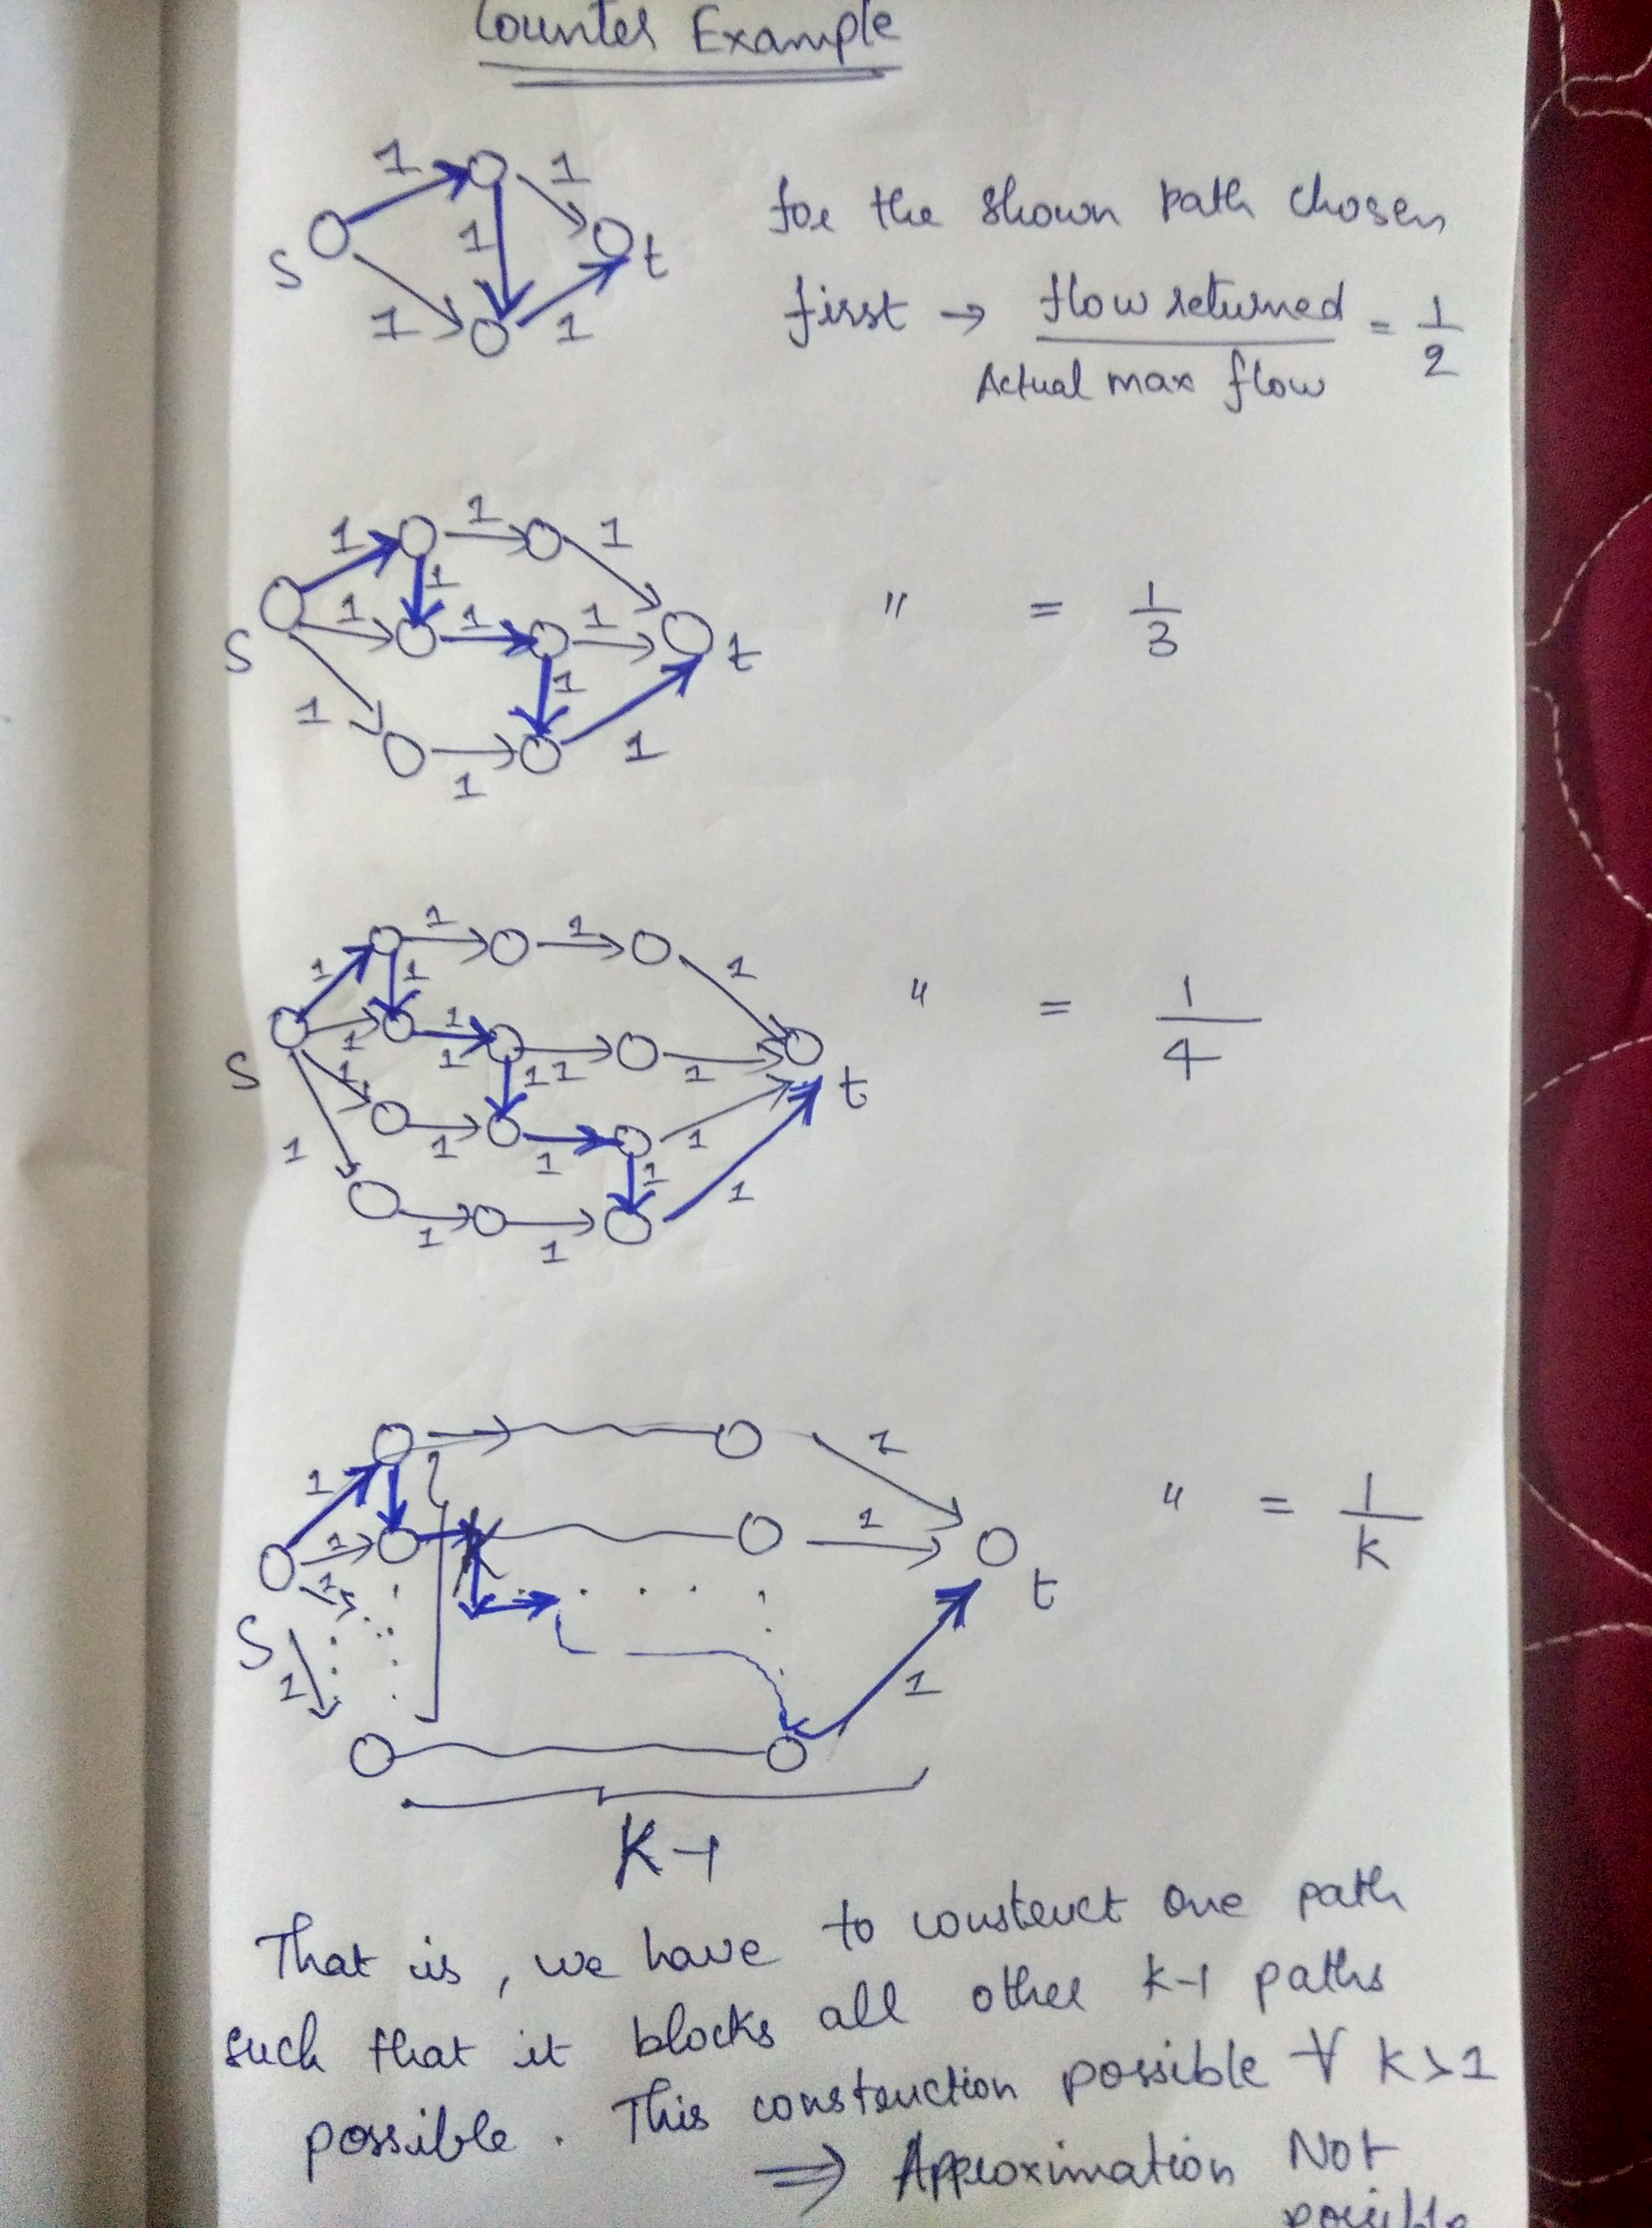
\includegraphics[scale=0.5]{1.jpg}
\newpage
\section{Locating faults in a network}
\subsection{Overview}
First we find k-edge disjoint paths of the given graph using the max-flow application discussed in class. Call these $\{p_1, p_2, .., p_k\}$. For all $i$, we pick $p_i$ and ping its middle vertex. If the result is true, we know that all the vertices to the left of this vertex will also be connected to $S$. If the result is false, we know that all the vertices to the right of this vertex will also be disconnected from $S$. Hence, at the end we get vertices marked connected/disconnected from vertex $S$. {\bf Notice only $O(klog(n))$ pings are issued in the process.}     

\subsection{Pseudo-Code}
\begin{algorithmic}[1]
  \Procedure{\textbf{findConnected}(V, E, s, t)}{}
  \State $\{p_1,p_2,..,p_k\} \gets$ k-disjoint paths between $s-t$ in $(V,E)$
  \State $S = \phi$
  \For{$i$ in $\{1,..,k\}$}
  \State $Nodes \gets$ nodes lying on path $p_i$ in the order of $s-t$
  \While{$Nodes <> NULL$}
  \If {$ping(Nodes[mid]) == TRUE$}
  \State $ S = S \cup Nodes[1..mid]$
  \State $ Nodes = Nodes[mid+1..last]$
  \Else
  \State $ Nodes = Nodes[1..mid-1]$
  \EndIf
  \EndWhile
  \EndFor
  \State return S
  \EndProcedure
\end{algorithmic} 
\subsection{Proof of Correctness}
\subsubsection{Claim: Every disjoint path has exactly one defaulted edge}
\subsubsection{Arguments}
\begin{itemize}
\item We are given k edge-disjoint paths from $s-t$.
\item It is also given that there is no functional path from $s-t$.
\item Hence, every edge-disjoint path should have atleast one defaulted edge otherwise $s-t$ will become connected which will be a contradiction.
\item As there are exactly k defaulted edges in total, from above we get that every disjoint path has exactly one defaulted edge.
\end{itemize} 
\subsubsection{Claim: Along any edge-disjoint path ping command will produce True,..,True, False,..False}
\subsubsection{Arguments}
\begin{itemize}
\item Any path starts with $s$ where $ping(s) = True$ is given.
\item Any path ends with $t$ where $ping(t) = False$ is given.
\item If the above said output is not produced by ping commands along a path then, there should be two distinct consecutive pairs of nodes in the path whose ping command should produce True, False. 
\item A True,False pair can occur consecutively only if these two vertices have a defaulted edge connecting them.
\item Therefore, if $3$ happened then there should be two defaulted edges in a given path, which is a contradiction from the previous claim. This proved this claim.
\end{itemize}    
{\bf From the previous claim we have the ping pattern True,..,True,False,..,False along any path. This ensures the termination as well as the correctness of the binary search along any path.}
\newpage
\section{A max flow application}
\subsection{Without Extra Constraint}
\subsubsection{Overview}
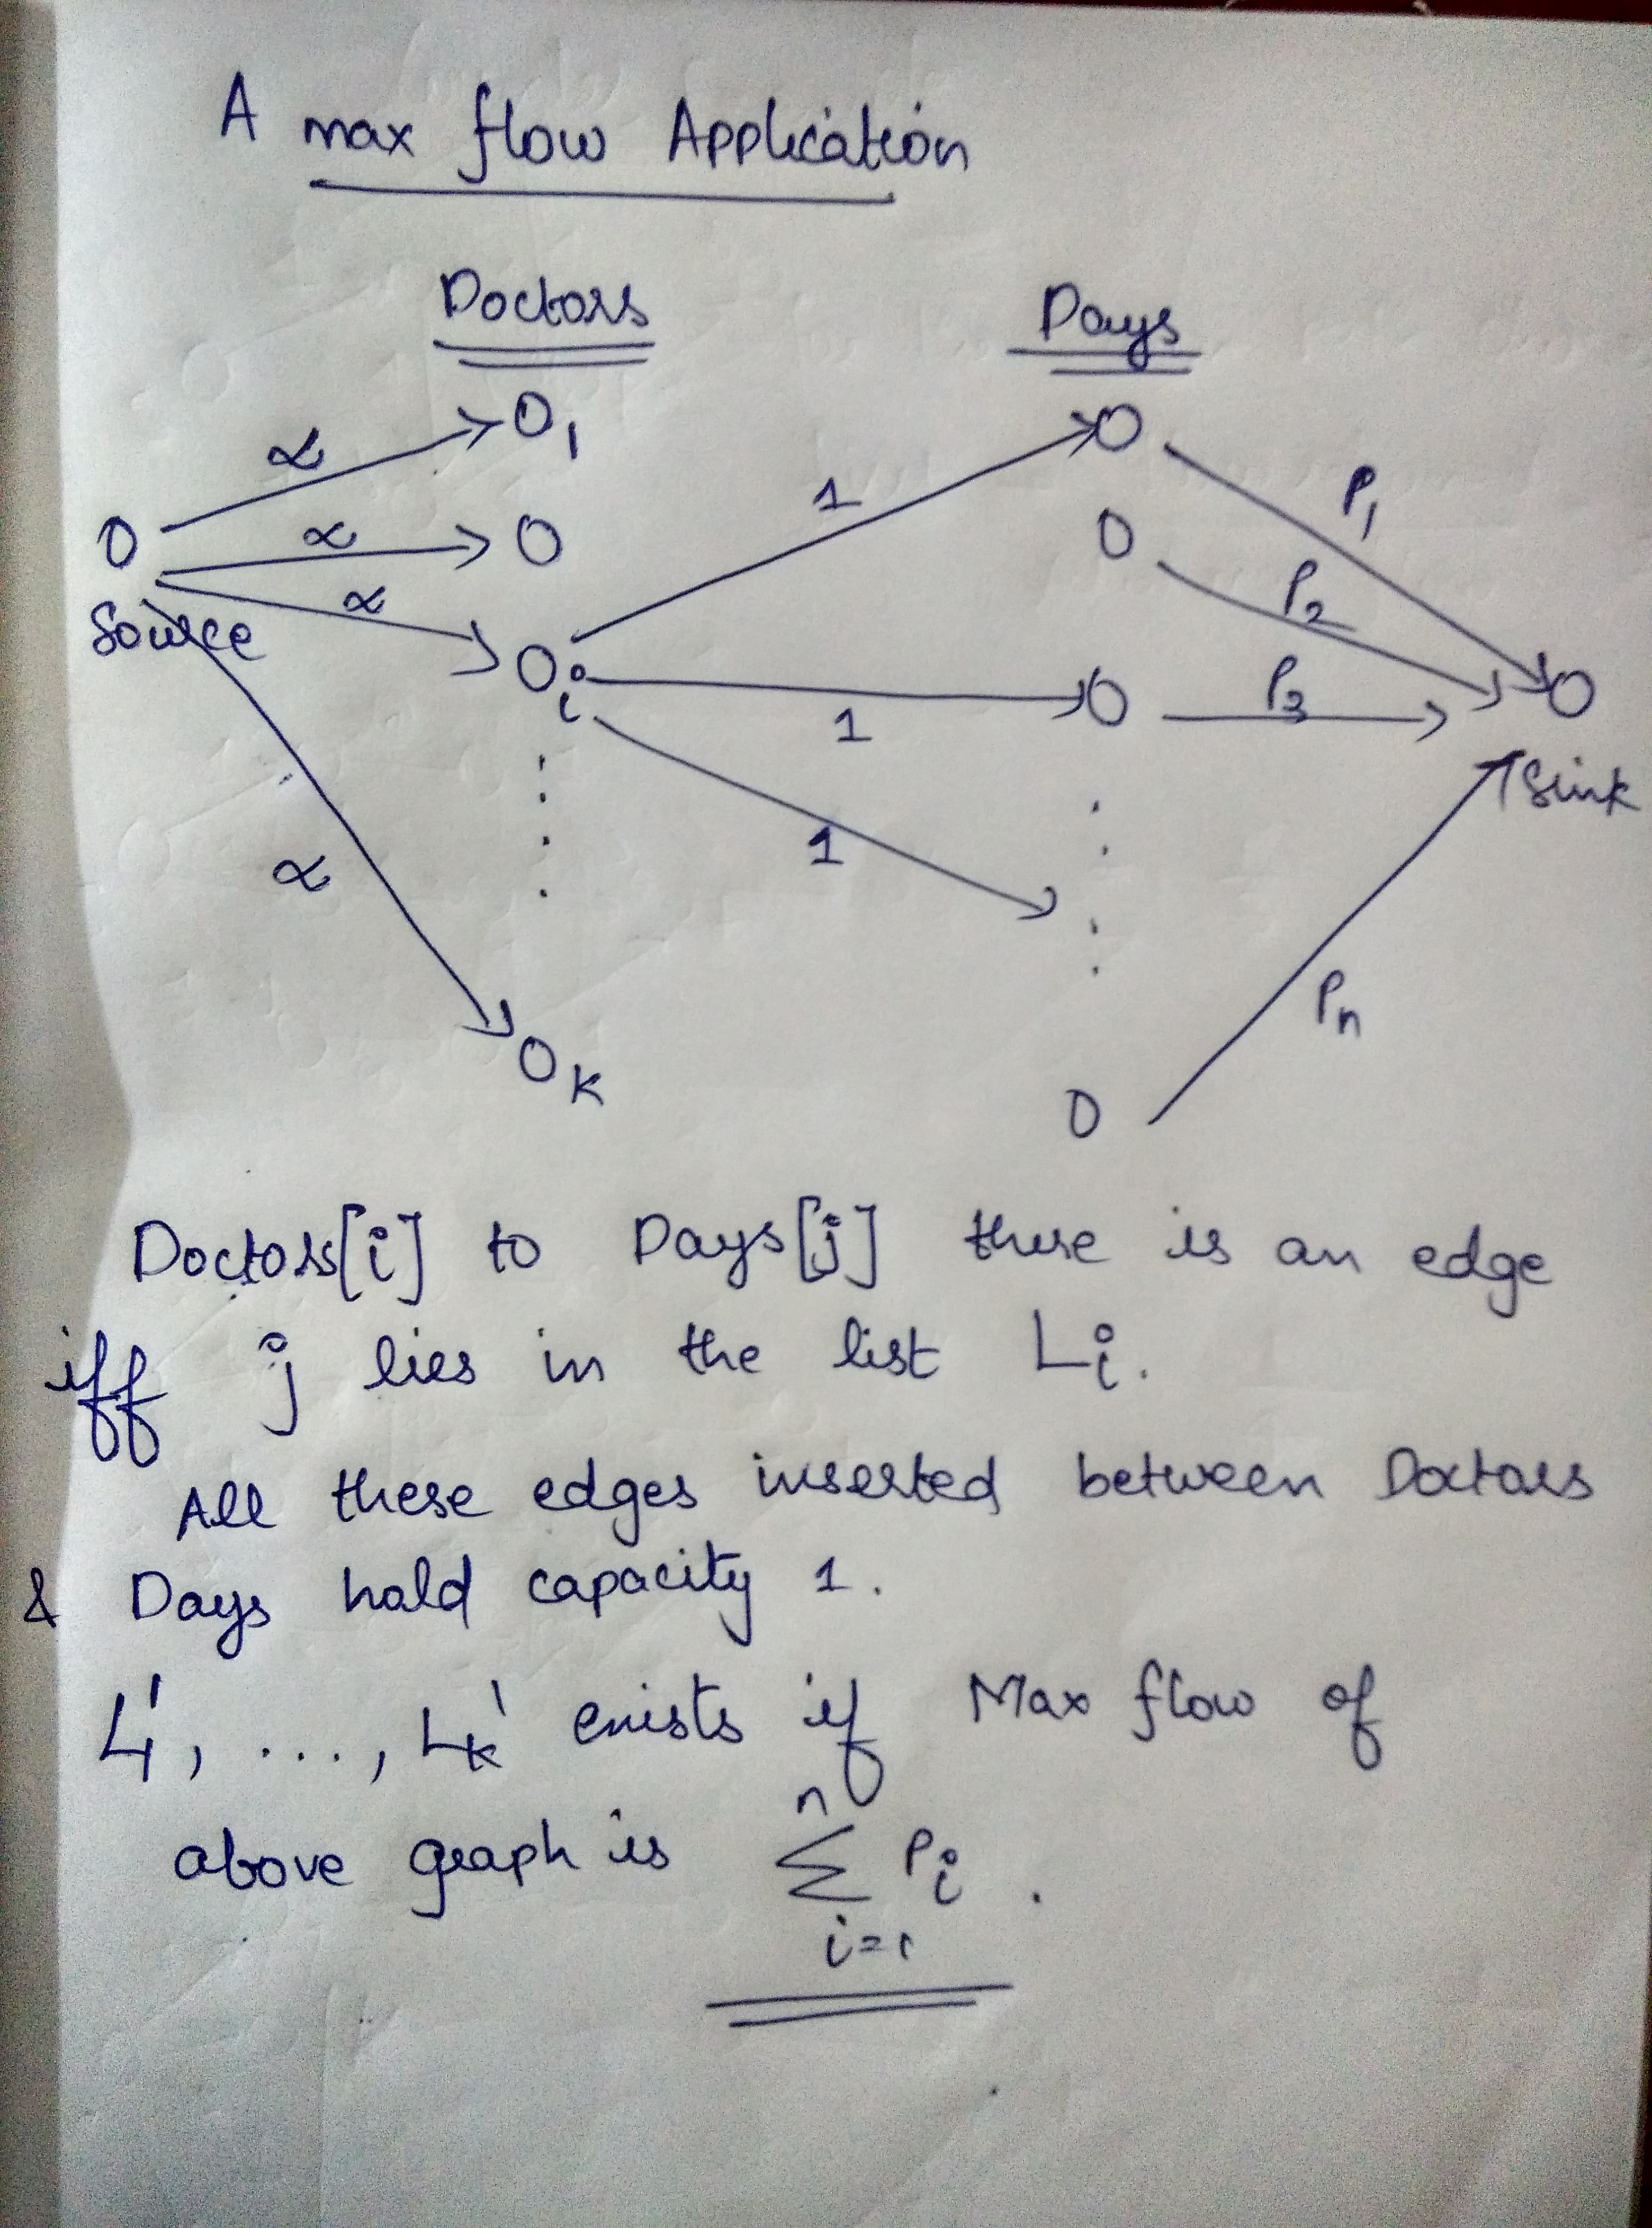
\includegraphics[scale=0.15]{3a.jpg}
\subsubsection{Notations}
$p_i$ denotes the exact number of doctors required on day $i$ \\
$L_i$ denotes the list of days where doctor $i$ is available \\
$L'_i$ denotes the list of days that doctor $i$ has to work to produce the required match. Note, $L'_i \subseteq L_i$\\
$D = \sum_{i=1}^{n} p_i$ \\
$n$ = Number of days in total \\
$k$ = Number of Doctors in total \\ 
\subsubsection{Claim}
Construction of $L'_i$s is possible if and only if the max-flow in the source-sink graph constructed (in image) is D.
\subsubsection{Proof - Part 1}
{\bf Given $L'_i$s list for all doctors, show that the max flow of source-sink graph shown above is D \\}
Construct a flow $f$ of the source-sink graph as follows. \\
$f(source,Doctor[i])$ is $|L'_i|$ - satisfies capacity constraint as these edges had infinite capacity \\
$f(Doctor[i], Day[j])$ is $1$ if $j$ lies in $L'_i$, otherwise is $0$ - satisfies capacity constraint \\
$f(Day[j],sink)$ is $p_j$ - satisfies capacity constraint \\
Flow Conservation is ensured as it is given to us that $L'_i$s of such definitions exist. \\
Hence, the above is a valid flow. \\
As the $cut-capacity$ between $sink$ and the rest of the graph is $D$, by $min-cut - max-flow$ theorem, $f$ should be a max flow of the source-sink graph. Hence, proved. 
\subsubsection{Proof - Part 2}
{\bf Given the max flow of source-sink graph to be D, show that $L'_i$s list for all doctors exist \\}
Let $f$ be the integral max-flow of the source-sink graph. (Note: Integral flow exists was proved in class) \\
Construct $L'_i$ as follows. \\
If $f(Doctor[i], Day[j])$ is $1$ then add $j$ to $L'_i$ otherwise do nothing. \\
Note: $f(Doctor[i], Day[j])$ can be only $0$ or $1$ by integral flow property. \\
The $L'_i$s thus constructed are valid as $value(f) = D$ implying every day $j$ has got the exact number of doctors wanted ($p_j$). Moreover, $L'_i \subseteq L_i$ is ensured from the construction of the source-sink graph itself. Hence, proved.
\newpage
\subsection{With Extra Constraint}
\subsubsection{Overview}
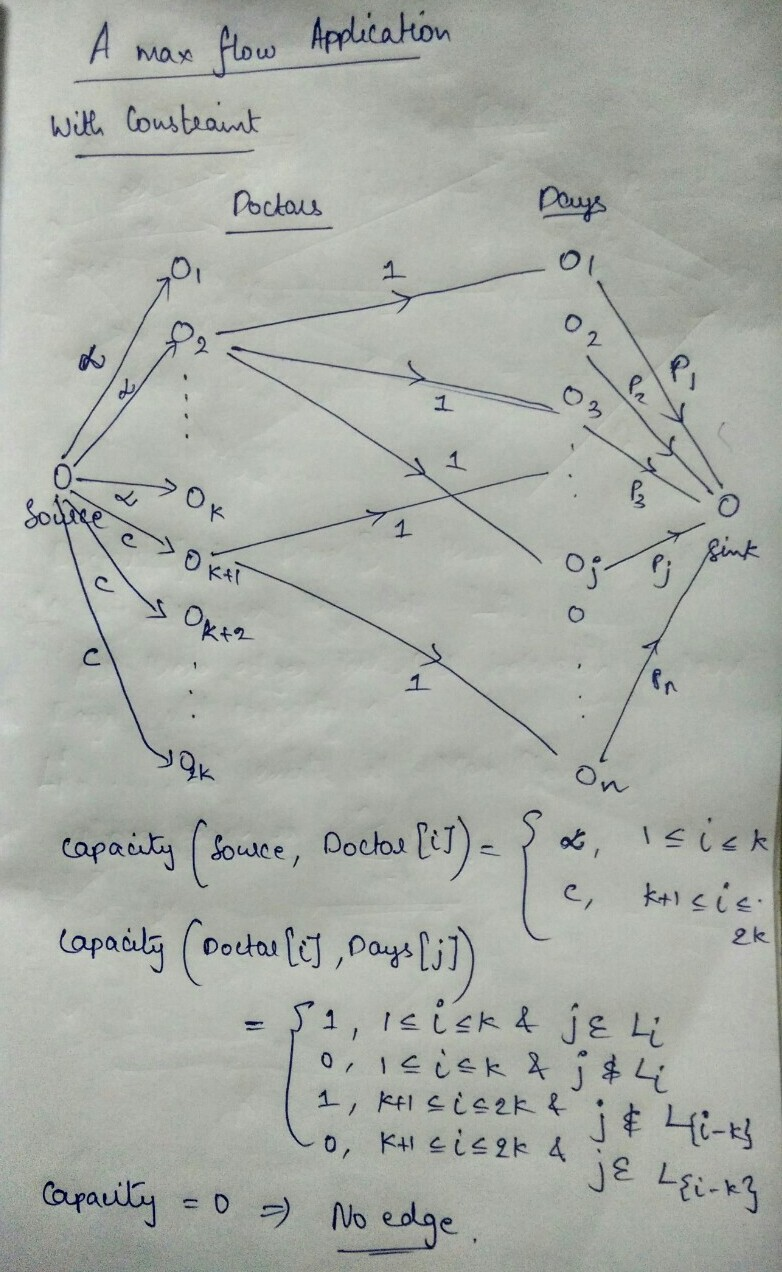
\includegraphics[scale=0.5]{3b.jpg}
\newpage
\subsubsection{Notations}
$p_i$ denotes the exact number of doctors required on day $i$ \\
$L_i$ denotes the list of days where doctor $i$ is available \\
$L'_i$ denotes the list of days that doctor $i$ has to work to produce the required match. \\
$K_i = L_i \cap  L'_i$ \\
$C_i = L'_i - K_i$ \\ 
$D = \sum_{i=1}^{n} p_i$ \\
$n$ = Number of days in total \\
$k$ = Number of Doctors in total \\ 
\subsubsection{Claim}
Construction of $L'_i$s is possible if and only if the max-flow in the source-sink graph constructed (in image) is D.
\subsubsection{Proof - Part 1}
{\bf Given $L'_i$s list for all doctors, show that the max flow of source-sink graph shown above is D \\}
Construct a flow $f$ of the source-sink graph as follows. \\
If $i \leq k$ then \\
$f(source,Doctor[i])$ is $|K_i|$ - satisfies capacity constraint as these edges had infinite capacity \\
$f(Doctor[i], Day[j])$ is $1$ if $j$ lies in $K_i$, otherwise is $0$ - satisfies capacity constraint \\
If $i > k$ then \\
$f(source,Doctor[i])$ is $|C_i|$ - satisfies capacity constraint by definition of $L'_i$s existence. \\
$f(Doctor[i], Day[j])$ is $1$ if $j$ lies in $C_i$, otherwise is $0$ - satisfies capacity constraint \\
 \\
$f(Day[j],sink)$ is $p_j$ - satisfies capacity constraint \\
 \\
Flow Conservation is ensured as it is given to us that $L'_i$s of such definitions exist. \\
Hence, the above is a valid flow. \\
As the $cut-capacity$ between $sink$ and the rest of the graph is $D$, by $min-cut - max-flow$ theorem, $f$ should be a max flow of the source-sink graph. Hence, proved. 
\subsubsection{Proof - Part 2}
{\bf Given the max flow of source-sink graph to be D, show that $L'_i$s list for all doctors exist \\}
Let $f$ be the integral max-flow of the source-sink graph. (Note: Integral flow exists was proved in class) \\
Construct $L'_i$ as follows. \\
If $f(Doctor[i], Day[j])$ or $f(Doctor[i+k], Day[j])$ is $1$ then add $j$ to $L'_i$ otherwise do nothing. \\
Note: $f(Doctor[i], Day[j])$ can be only $0$ or $1$ by integral flow property. \\
The $L'_i$s thus constructed are valid as $value(f) = D$ implying every day $j$ has got the exact number of doctors wanted ($p_j$). Moreover, both $f(Doctor[i], Day[j])$ and $f(Doctor[i+k], Day[j])$ will not be together $1$ from the construction of source-sink graph itself. Hence, proved.
\end{document}